\chapter{Samples}

\begin{defn}[ver \cite{Dodd2005}] Definición definitiva $$\frac{d}{dx}\int_a^xf(y)dy=f(x).$$\end{defn}

\begin{enumerate}
	\item Item 1
	\begin{enumerate}
		\item Subitem 1
		\item Subitem 2 (ver Figura \ref{logofcfm})
	\end{enumerate}
	\item Item 2
	\item Item 3
\end{enumerate}
\begin{teo}
	Se tiene más que $$\int_0^t e^sds=e^t-1.$$
\end{teo}

\begin{figure}[!h]
	\centering
	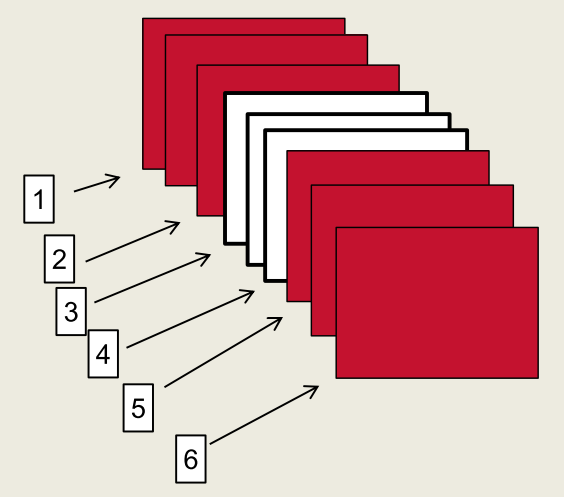
\includegraphics[scale=.2]{eventos.png}
	\caption{Logo de la Facultad}
	\label{logofcfm}
\end{figure}

\begin{table}[!h]
	\centering
	\begin{tabular}{|c||c|}
		\hline
		Campo 1& Campo 2\\\hline
		Valor 1& Valor2\\\hline
	\end{tabular}
	\caption{Tabla 1}
	\label{tabla:1}
\end{table}

\lipsum[36-40]